% \CheckSum{622}
%
% \iffalse meta-comment
% Files `tabvar.dtx’, `tabvar.ins’ and `tabvar.mp’
%
% Copyright (C) Daniel Flipo 2003-2022 <daniel.flipo at free.fr>
%
% All the files included in the `tabvar’ distribution, including
% the font, may be distributed and/or modified under the conditions
% of the LaTeX Project Public License, either version 1.3 of this
% license or (at your option) any later version.
% The latest version of this license is in
%    http://www.latex-project.org/lppl.txt
% and version 1.3 or later is part of all distributions of LaTeX
% version 2003/12/01 or later.
%
% This file has the LPPL maintenance status `maintained’.
%
% \fi
%
% \iffalse
%
%<*sty>
%%
%% Copyright (C) Daniel Flipo 2003-2022 <daniel.flipo at free.fr>
%%
\NeedsTeXFormat{LaTeX2e}[1997/06/01]
\ProvidesFile{tabvar.sty}
%</sty>
%<*dtx>
\ProvidesFile{tabvar.dtx}
%</dtx>
%<*!cfg>
             [2022/07/16 v1.8 (Daniel Flipo)]
%</!cfg>
%
%<*driver>
\documentclass[a4paper]{ltxdoc}
\usepackage{tabvar}
\GetFileInfo{tabvar.dtx}
\RecordChanges
%\OnlyDescription
%
\usepackage{iftex,url}
\iftutex
  \usepackage{fontspec}
\else
  \usepackage[T1]{fontenc}
  \usepackage{lmodern}
\fi
\usepackage[french]{babel}
\GlossaryPrologue{\section*{Historique des versions}}
\newcommand*\file[1]{\textsf{#1}}
\newcommand*\ctype[1]{\texttt{#1}}
\newcommand*\env[1]{\texttt{#1}}
\setlength{\parindent}{0pt}
\setlength{\parskip}{.5\baselineskip plus .2\baselineskip
                                     minus .2\baselineskip}
\begin{document}
\begin{center}
  \textbf{\Large Tableaux de variations : `tabvar’}\\[3mm]^^A\]
  Daniel \textsc{Flipo}\\
  \texttt{Daniel.Flipo\at free.fr}
\end{center}
 \DocInput{tabvar.dtx}
\end{document}
%</driver>
%
% \fi
%
%  \section{Documentation}
%
%    L’extension \file{tabvar.dtx}\footnote{La version présentée
%    ici porte le numéro \fileversion, dernière modification le
%    \filedate.}, a pour but de faciliter la saisie des tableaux de
%    variations. Elle fonctionne aussi bien avec pdfLaTeX qu’avec
%    LuaLaTeX ou XeLaTeX.
%
%    Elle s’appuie sur les extensions \file{array}, \file{colortbl},
%    et \file{varwidth}. Les flèches sont prises dans une fonte
%    (type\,1) spécialement créée par Michel~\bsc{Bovani}.
%    Depuis la version~1.5, quatre variantes de flèches sont
%    proposées.
%    Un grand merci à Michel pour cette contribution et pour
%    ses remarques qui m’ont été très utiles pour
%    améliorer les versions préliminaires.
%
%    Une autre possibilité (conservée uniquement pour préserver
%    la compatibilité avec les premières versions de \file{tabvar})
%    consiste à faire appel, pour le dessin des flèches,
%    à MetaPost : le fichier \file{tabvar.mp} permet de créer les
%    trois flèches \file{tabvar.1}, \file{tabvar.2}, \file{tabvar.3}.
%    Ceci est une solution de repli pour ceux qui auraient du mal
%    à installer la fonte \file{tabvar.pfb}, à n’employer qu’en
%    dernier recours.
%
%  \subsection{Installation}
%
%    L’extension \file{tabvar} fait partie des distributions TeXLive,
%    MacTeX, ProTeXt, MikTeX, etc. Si elle n’est pas installée chez
%    vous, assurez-vous d’abord que l’extension \file{varwidth.sty} est
%    présente sur votre système, sinon récupérez-la sur CTAN :
%    cherchez par exemple la chaîne |varwidth|
%    sur \url{http://www.tex.ac.uk/CTANfind.html}
%
%    Les fichiers \file{tabvar.1}, \dots{} , \file{tabvar.3}
%    ainsi que \file{tabvar.sty} et \file{tabvar.cfg} doivent
%    être placés dans un répertoire vu par \LaTeX.
%
%    Les flèches sont prises dans la fonte type\,1 \file{tabvar.pfb}
%    à condition que celle-ci soit correctement installée :
%    il est nécessaire de placer le fichier \file{tabvar.pfb} dans
%    un répertoire où il sera pris en compte, par exemple, pour
%    respecter l’architecture TDS : |texmf/fonts/type1/public/tabvar|.
%    De même, son fichier de métriques \file{tabvar.tfm} devra
%    être mis par exemple dans |texmf/fonts/tfm/public/tabvar|.
%
%    Un ligne donnant accès à cette fonte doit être ajoutée
%    (voir \file{tabvar.map}) dans les fichiers |.map| utilisés
%    par le pilote PostScript (\file{psfonts.map}) et par pdf\TeX{}
%    (\file{pdftex.map}).
%    Ne pas oublier de mettre à jour les bases de données ls-R
%    pour terminer (commande |mktexlsr| sous te\TeX{} ou \TeX{}Live).
%
%  \subsection{Utilisation}
%
%    L’environnement \env{tabvar} est une variante de l’environnement
%    |array|, adaptée à la saisie de tableaux de variations.
%
%    Trois nouveaux types de colonnes, \ctype{C}, \ctype{L} et
%    \ctype{R} remplacent les types classiques \ctype{c}, \ctype{l}
%    et \ctype{r} ; ils permettent de disposer du matériel sur
%    plusieurs niveaux dans un même ligne du tableau (ce sont des
%    colonnes de type |\parbox|).
%
%    Un quatrième type de colonne, noté \ctype{U}%
%    \footnote{Il était noté \ctype{N} jusqu’à la version~1.5,
%    le type \ctype{N} est conservé pour assurer la
%    compatibilité ascendante mais ne devrait plus être utilisé
%    pour éviter un conflit avec l’extension \file{numprint.sty}.}
%    sert pour les plages où la fonction n’est pas définie
%    (\ctype{U} pour \textit{Undefined}). La colonne est entièrement
%    grisée par défaut, mais il est possible de choisir une autre
%    couleur (voir le fichier de configuration \file{tabvar.cfg}).
%    Désormais \file{tabvar} teste au |\begin{document}| si le type
%    \ctype{N} a été défini par une autre extension, si c’est le
%    cas un avertissement est affiché dans le fichier \file{.log} et
%    \file{tabvar} n’écrase plus la définition du type \ctype{N}.
%    Sinon, le type \ctype{N} est défini comme avant.
%
%    La saisie des lignes contenant les valeurs de la variable et les
%    signes des dérivées se fait exactement comme celles d’un
%    tableau |array|. Seules les lignes contenant les variations de
%    la ou des fonctions font appel à six commandes
%    particulières : |\niveau|, |\croit|, |\decroit|, |\constante|,
%    |\dbarre| et |\discont|.
%
%    \begin{itemize}
%
%      \item |\niveau{|\emph{départ}|}{|\emph{total}|}| prend
%        deux arguments : le niveau (hauteur) où doit être
%        positionnée la première valeur de la fonction et le
%        nombre total de niveaux qui seront utilisés dans la ligne.
%        Le niveau le plus bas est numéroté 1.
%
%      \item Les commandes |\croit|, |\decroit| et |\constante| ne
%        prennent pas d’argument, elles tracent les flèches
%        montantes, descendantes ou horizontales.
%
%      \item |\dbarre| trace un double trait vertical dont la hauteur
%        est celle de la ligne du tableau ; elle indique les
%        discontinuités de la fonction.
%
%      \item |\discont[|\emph{num}|]{|\emph{valeur\_gauche}|}{<|
%        ou |>}{|\emph{valeur\_droite}|}| peut
%        s’utiliser lorsque la fonction présente une
%        discontinuité à la place de la double barre
%        traditionnelle ; elle prend trois arguments obligatoires :
%        les valeurs à gauche~$f_-$ et à droite~$f_+$ de la
%        fonction, séparées par un signe |<| ou |>| selon que
%        $f_-<f_+$ ou $f_->f_+$.
%        Enfin, l’argument optionnel, qui vaut~0 par défaut,
%        permet d’intercaler \emph{num} niveaux supplémentaires
%        entre les valeurs de~$f_-$ et~$f_+$ si nécessaire.
%
%    \end{itemize}
%
%    Il est possible d’ajouter des filets d’alignement vertical en
%    utilisant la commande |\barre{}| qui requiert un argument
%    obligatoire, éventuellement vide : |\barre{}| trace un filet
%    vertical dont la hauteur est celle de la ligne du tableau.
%    Lorsqu’une valeur doit figurer sous le filet, on la passe en
%    argument de la commande (|\barre{0}| par exemple), ainsi cette
%    valeur sera centrée sur le filet.  Ceci restreint évidemment
%    l’usage de la commande |\barre| aux colonnes de type \ctype{C}.
%    La couleur du filet (gris par défaut) est paramétrable, voir
%    le fichier de configuration \file{tabvar.cfg}. Cette solution a
%    été préférée à des pointillés qui posent des
%    problèmes de raccordement d’une ligne à l’autre du tableau.
%
%    Depuis la version 1.5, quatre variantes sont proposées pour le
%    dessin des flèches PostScript type\,1, elles sont accessibles
%    par les commandes |\FlechesPS1| (flèches «à moustaches»
%    obtenues par défaut), |\FlechesPS2| (assorties à la police
%    Fourier), |\FlechesPS3| et |\FlechesPS4|.
%
%    La commande |\TVcenter| prend un argument, elle sert à
%    centrer verticalement le nom de la fonction, par exemple
%    |\TVcenter{f(x)}|. Elle a besoin de connaître le nombre
%    total de niveaux, elle doit donc être précédée d’une
%    commande |\niveau{|\emph{départ}|}{|\emph{total}|}|.
%
%    La commande |\TVstretch| est à utiliser lorsqu’un élément
%    du tableau colle à la ligne horizontale du dessus ou du
%    dessous%
%    \footnote{Noter que les extensions \file{cellspace} et
%    \file{tabls} qui règlent ce problème n’ont pas d’effet
%    sur l’environnement \env{tabvar} et que \file{tabls} est
%    incompatible avec \file{array} chargé par \file{tabvar}.}.
%    |\TVstretch{|\emph{valeur}|}| ajoute un peu d’espace
%    paramétrable (2pt par défaut)%
%    \footnote{La valeur de l’espace ajouté au-dessus est définie
%    par \texttt{\boi setlength\{\boi TVextraheight\}\{2pt\}}, celle
%    de l’espace ajouté au-dessous est définie par
%    \texttt{\boi setlength\{\boi TVextradepth\}\{2pt\}}.}
%    au dessus et en dessous de \emph{valeur}.
%
%    La commande |\TVstretch| accepte un argument optionnel de type
%    \emph{dimension} qui s’utilise lorsqu’on souhaite n’ajouter
%    d’espace vertical que d’un côté (au-dessus ou au-dessous).
%    Si l’argument optionnel est une dimension positive, sa valeur
%    sera ajoutée uniquement au-dessus et si c’est une dimension
%    négative sa valeur absolue sera ajoutée uniquement en
%    dessous.
%
%    Le fichier \file{demo.pdf} (joint) propose plusieurs exemples,
%    accompagnés de leur code source, illustrant les utilisations
%    possibles de l’environnement \env{tabvar}.
%
%    Plusieurs commandes ou paramètres permettent de personnaliser
%    l’aspect du tableau (augmentation de la largeur ou de la hauteur
%    des cellules, etc.), voir le fichier \file{tabvar.cfg}.
%
%  \subsection{Incompatibilités}
%
%    \file{tabvar} est incompatible avec les extensions qui
%    définissent les mêmes types de colonnes (\ctype{C},
%    \ctype{L}, \ctype{R}, \ctype{U}) pour d’autres usages, en
%    particulier \file{tabulary}.
%
%    Lorsqu’on utilise l’extension \file{xcolor}, placer l’appel
%    à |\usepackage{xcolor}| \emph{avant} |\usepackage{tabvar}|,
%    afin d’éviter un certain nombre de \textit{Warnings}.
%
% \StopEventually{\PrintChanges}
%
% \iffalse
%<*sty>
% \fi
%
%  \section{Le code}
%
%  \subsection{Options}
%
% \changes{tabvar-0.9}{2004/12/29}{Par défaut, les flèches
%    sont prises maintenant dans la fonte type 1 de Michel Bovani.}
%
% \changes{tabvar-0.9}{2005/02/05}{Ajout de deux options pour
%    le choix du type de flèches (suggestion de Frank Stengel).}
%
%    Depuis la version~0.9, les flèches utilisées par défaut
%    sont prises dans la fonte type\,1 de Michel Bovani.
%
%    Si cette fonte spécifique n’a pas pu être correctement
%    installée, on pourra déclarer |\FlechesMPtrue| dans le
%    fichier \file{tabvar.cfg} ou dans le préambule, ou encore
%    utiliser l’option |FlechesMP| pour que les flèches
%    MetaPost utilisées à la place. Cette solution est à
%    proscrire lorsqu’on travaille avec XeLaTeX ou LuaLaTeX.
%
%    \begin{macrocode}
\newif\ifFlechesMP \FlechesMPfalse
\DeclareOption{FlechesMP}{\FlechesMPtrue}
\DeclareOption{FlechesPS}{\FlechesMPfalse}
\ProcessOptions
%    \end{macrocode}
%
%  \subsection{Identification, extensions requises}
%
%    Chargement des extensions utiles :
%
%    \begin{macrocode}
\RequirePackage{array}
\RequirePackage{colortbl}
\RequirePackage{varwidth}
\RequirePackage{ifthen}
%    \end{macrocode}
%
%  \subsection{Dessin des flèches}
%
%    Le fichier \file{tabvar.mp} (joint) contient le dessin des
%    trois flèches en MetaPost.
%
%    La commande |mpost -tex=latex tabvar| produit trois fichiers
%    \file{tabvar.1}\dots{} \file{tabvar.3} qui contiennent les
%    dessins des flèches ; en PDF, il faut indiquer qu’il s’agit
%    de fichiers MetaPost.
%
% \changes{tabvar-1.61}{2012/03/14}{Charger supp-pdf.tex est inutile :
%    en mode PDF, graphics.sty appelle pdftex.def qui charge
%    supp-pdf.mkii.}
%
%    \begin{macrocode}
\RequirePackage{graphicx}
\RequirePackage{ifpdf}
\ifpdf
  \DeclareGraphicsRule{*}{mps}{*}{}
\fi
%    \end{macrocode}
%
%\changes{tabvar-1.5}{2011/03/04}{La définition des flèches en
%  MetaPost est déplacée (AtBeginDocument) pour éviter un
%  message d’erreur avec XeLaTeX. Bug signalé par Thierry Wybrecht.}
%
%\changes{tabvar-1.2}{2008/10/23}{\cs{@ptsize} peut prendre des
%  valeurs négatives (classes koma-script avec tailles inférieures
%  à 10pt).  Utiliser \cs{f@size} à la place (patch proposé par
%  Ulrike Fisher, merci Ulrike).}
%
%    La mise à l’échelle des flèches MetaPost se fait à partir
%    de la valeur de |\f@size| qui contient normalement la taille en
%    points de la police de base (10 en 10pt). Si la classe utilisée
%    ne définit pas |\f@size|, on donne la valeur 10 à |\f@size|,
%    la valeur par défaut de |\TVarrowscale| est alors 1.0
%    (échelle 1), l’utilisateur peut toujours redéfinir lui-même
%    |\TVarrowscale| selon ses besoins.
%    \begin{macrocode}
\providecommand{\f@size}{10}
\newcommand{\TVarrowscale}{\strip@pt\dimexpr\f@size pt/10\relax}
%    \end{macrocode}
%
%\changes{tabvar-1.4}{2010/08/22}{Ajout d’une commande
%    \cs{TVarrowscolstretch} permettant d’augmenter la largeur des
%    colonnes contenant les flèches.}
%
%    La commande |\TVarrowscolstretch|, dont la valeur par défaut
%    est~1, permet d’augmenter la largeur des colonnes contenant les
%    flèches.
%
%  \begin{macro}{\TVarrowscolstretch}
%    \begin{macrocode}
\newcommand*{\TVarrowscolstretch}{1}
\newcommand*{\TV@arrowcol@stretch}[1]{%
     \makebox[\TVarrowscolstretch\width][c]{#1}}
%    \end{macrocode}
%  \end{macro}
%
%\changes{tabvar-1.5}{2011/03/10}{Trois nouvelles formes de flèches
%  déssinées par Michel Bovani.
%  Ajout de la commande \cs{FlechesPS} pour y accéder.}
%
%  La commande |\FlechesPS| suivie d’un chiffre compris entre 1 et 4
%  permet d’accéder à quatre variantes pour les flèches
%  PostScript.
%
%  \begin{macro}{\FlechesPS}
%    \begin{macrocode}
\newcommand*{\enearrow}{\enearrowi}
\newcommand*{\esearrow}{\esearrowi}
\newcommand*{\eastarrow}{\eastarrowi}
\newcommand*{\FlechesPS}[1]{%
  \renewcommand*{\enearrow}{%
    \csname enearrow\romannumeral#1\endcsname}%
  \renewcommand*{\esearrow}{%
    \csname esearrow\romannumeral#1\endcsname}%
  \renewcommand*{\eastarrow}{%
    \csname eastarrow\romannumeral#1\endcsname}%
}
%    \end{macrocode}
%  \end{macro}
%
%  \begin{macro}{\FlecheC}
%  \begin{macro}{\FlecheD}
%  \begin{macro}{\FlecheH}
%    Le tracé des trois types de flèches est fait par les
%    commandes |\FlecheC|, |\FlecheD| et |\FlecheH|. Le choix de la
%    variante (MetaPost ou type\,1) est fait au |\begin{document}|,
%    ce qui économise une fonte mathématique parmi les 16
%    disponibles lorsqu’on choisit la variante MetaPost.
%    \begin{macrocode}
\AtBeginDocument{%
  \ifFlechesMP
    \newsavebox{\arup}%
    \newsavebox{\ardown}%
    \newsavebox{\arhor}%
    \sbox{\arup}{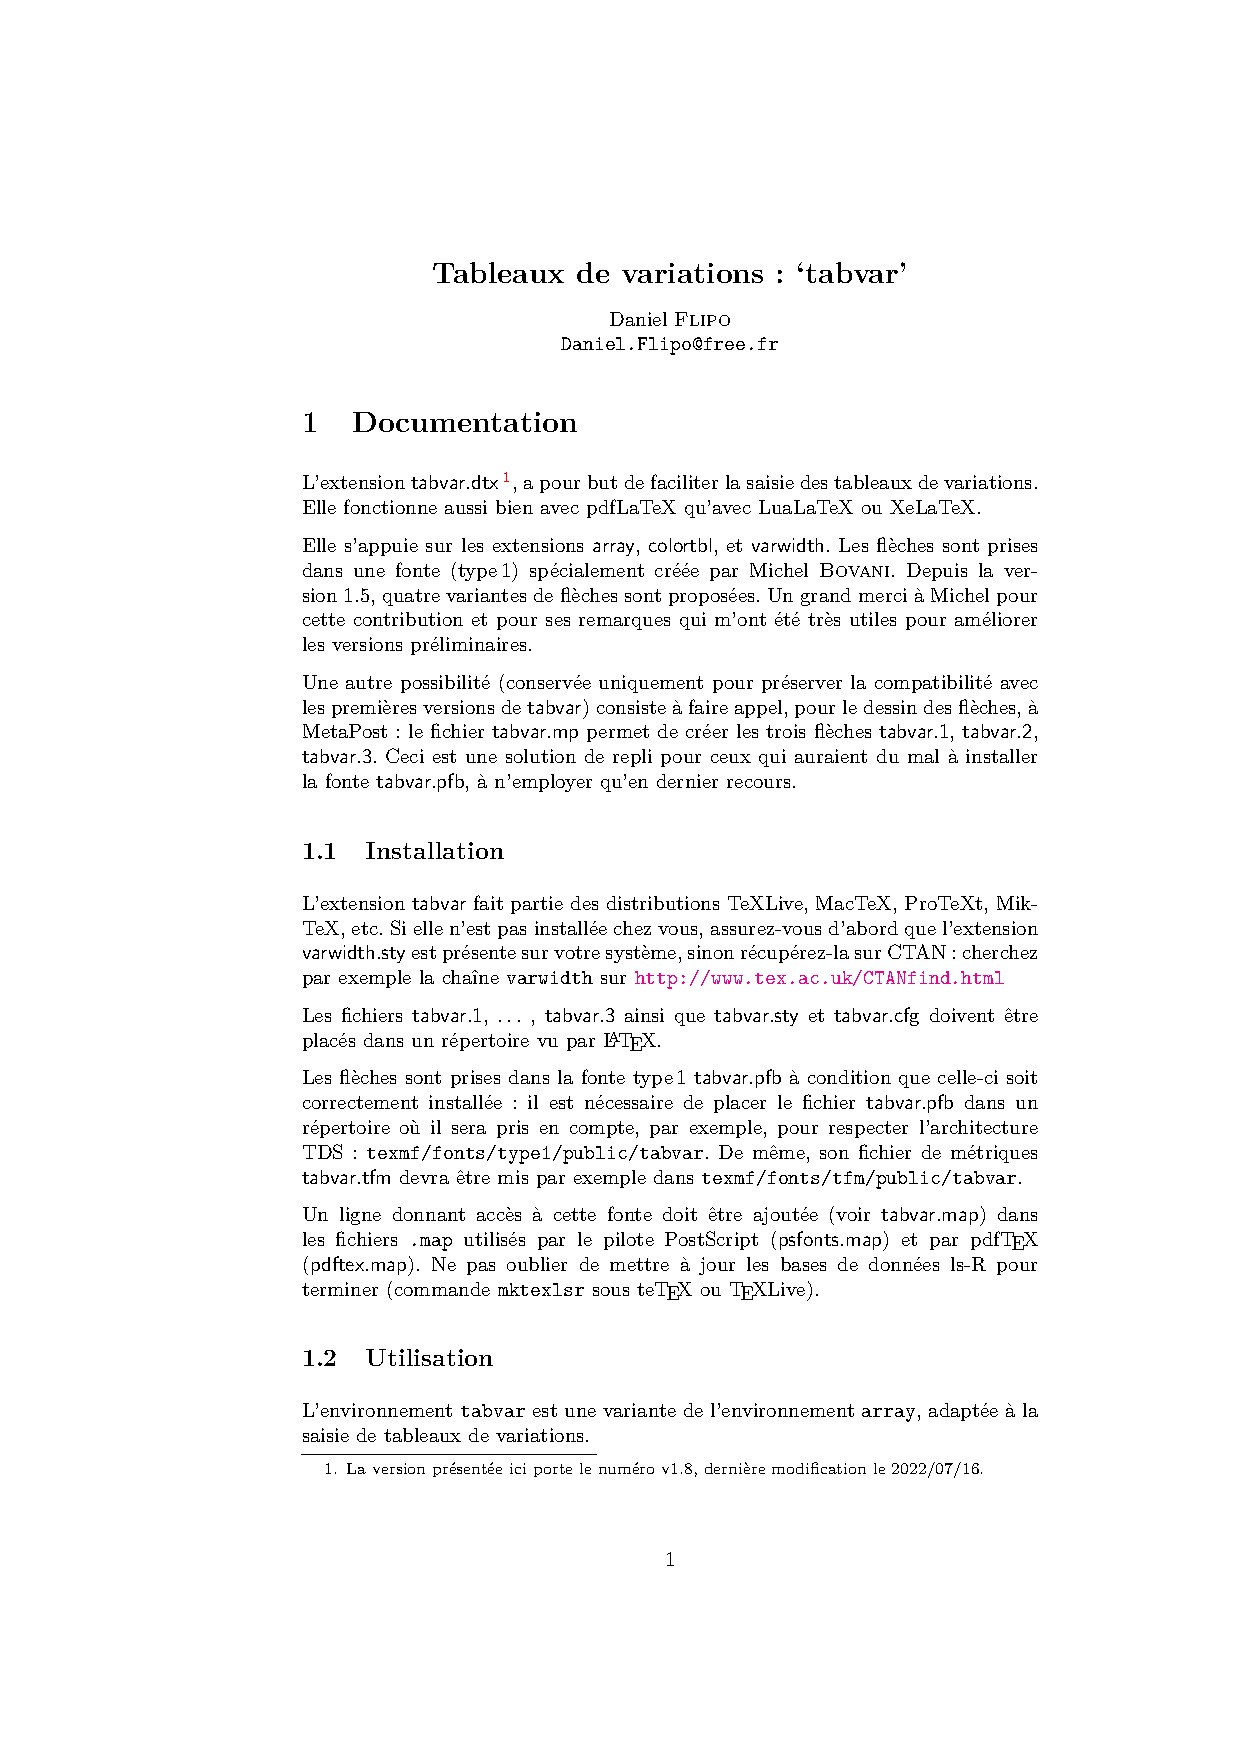
\includegraphics[scale=\TVarrowscale]{tabvar.1}}%
    \sbox{\ardown}{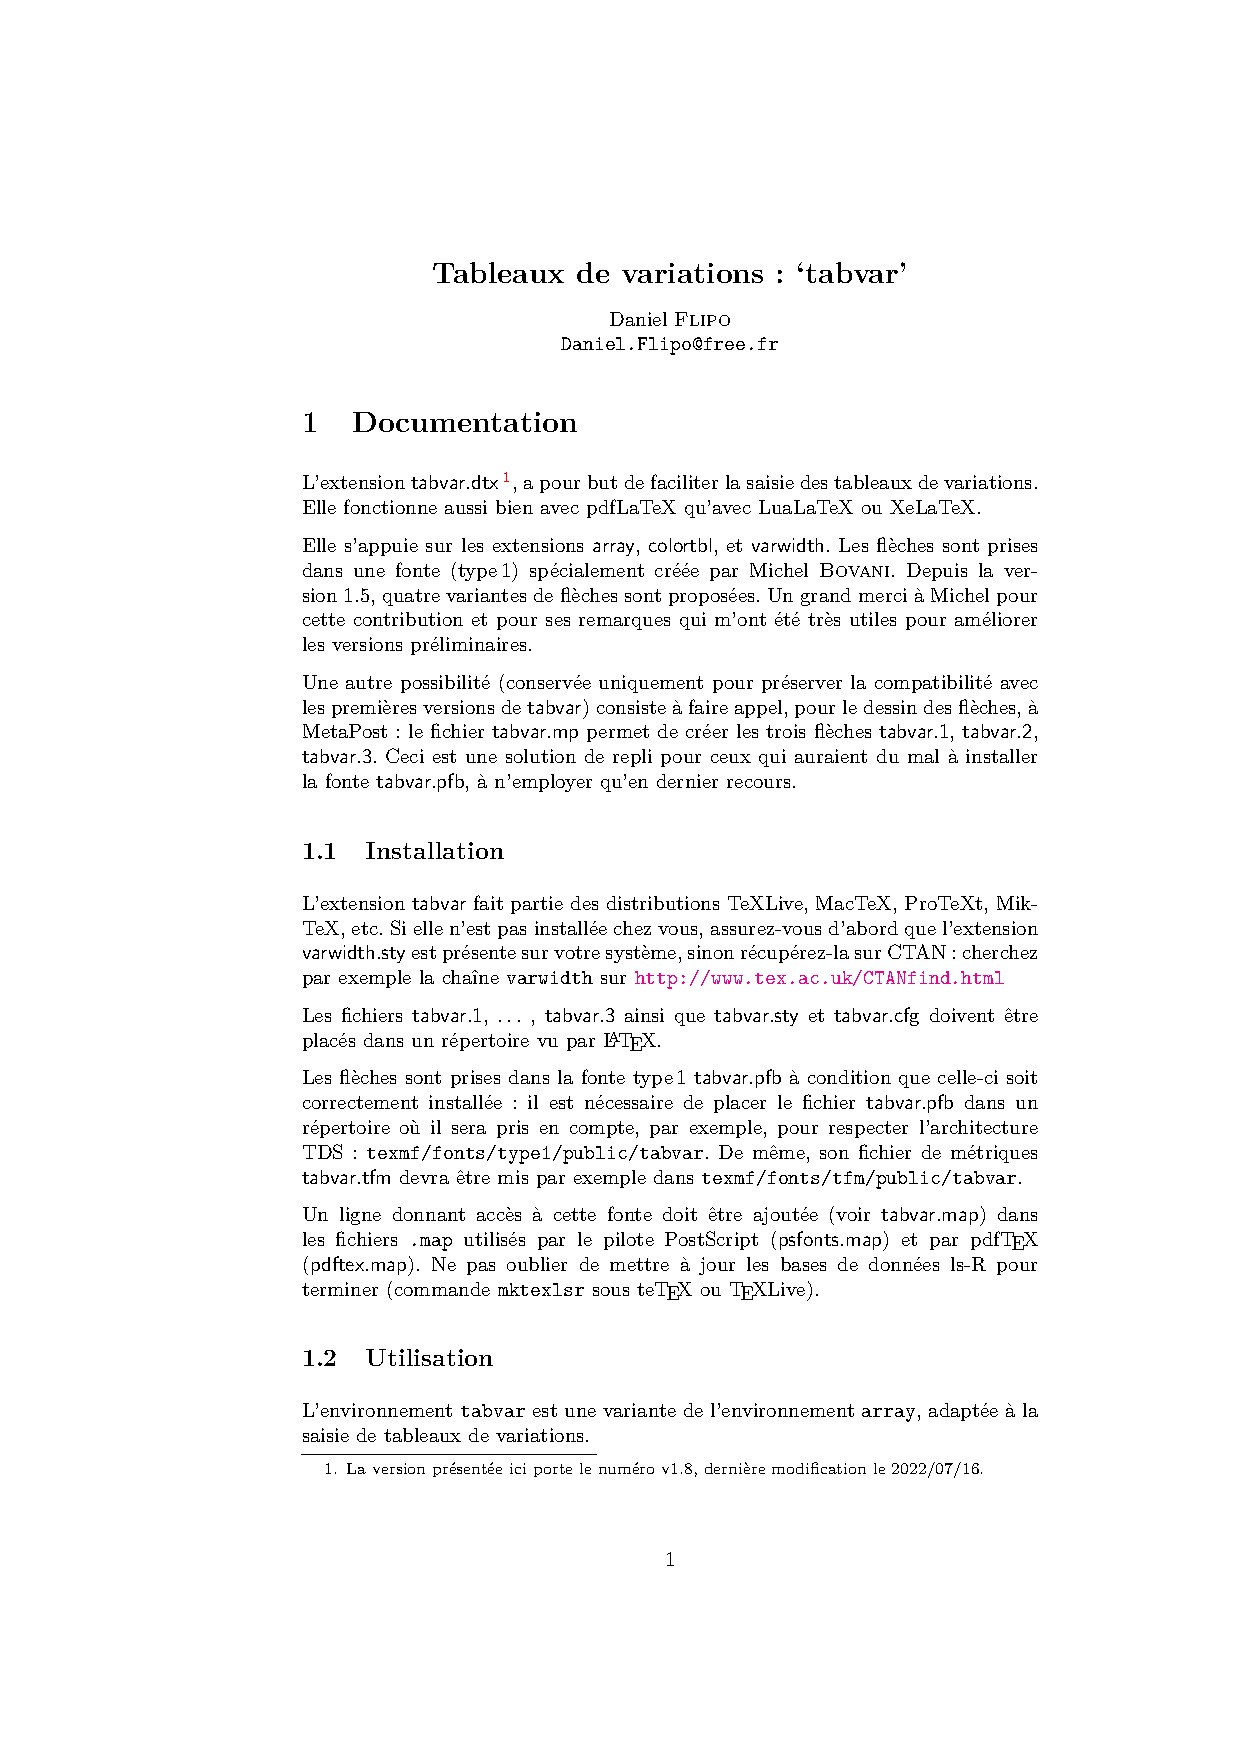
\includegraphics[scale=\TVarrowscale]{tabvar.2}}%
    \sbox{\arhor}{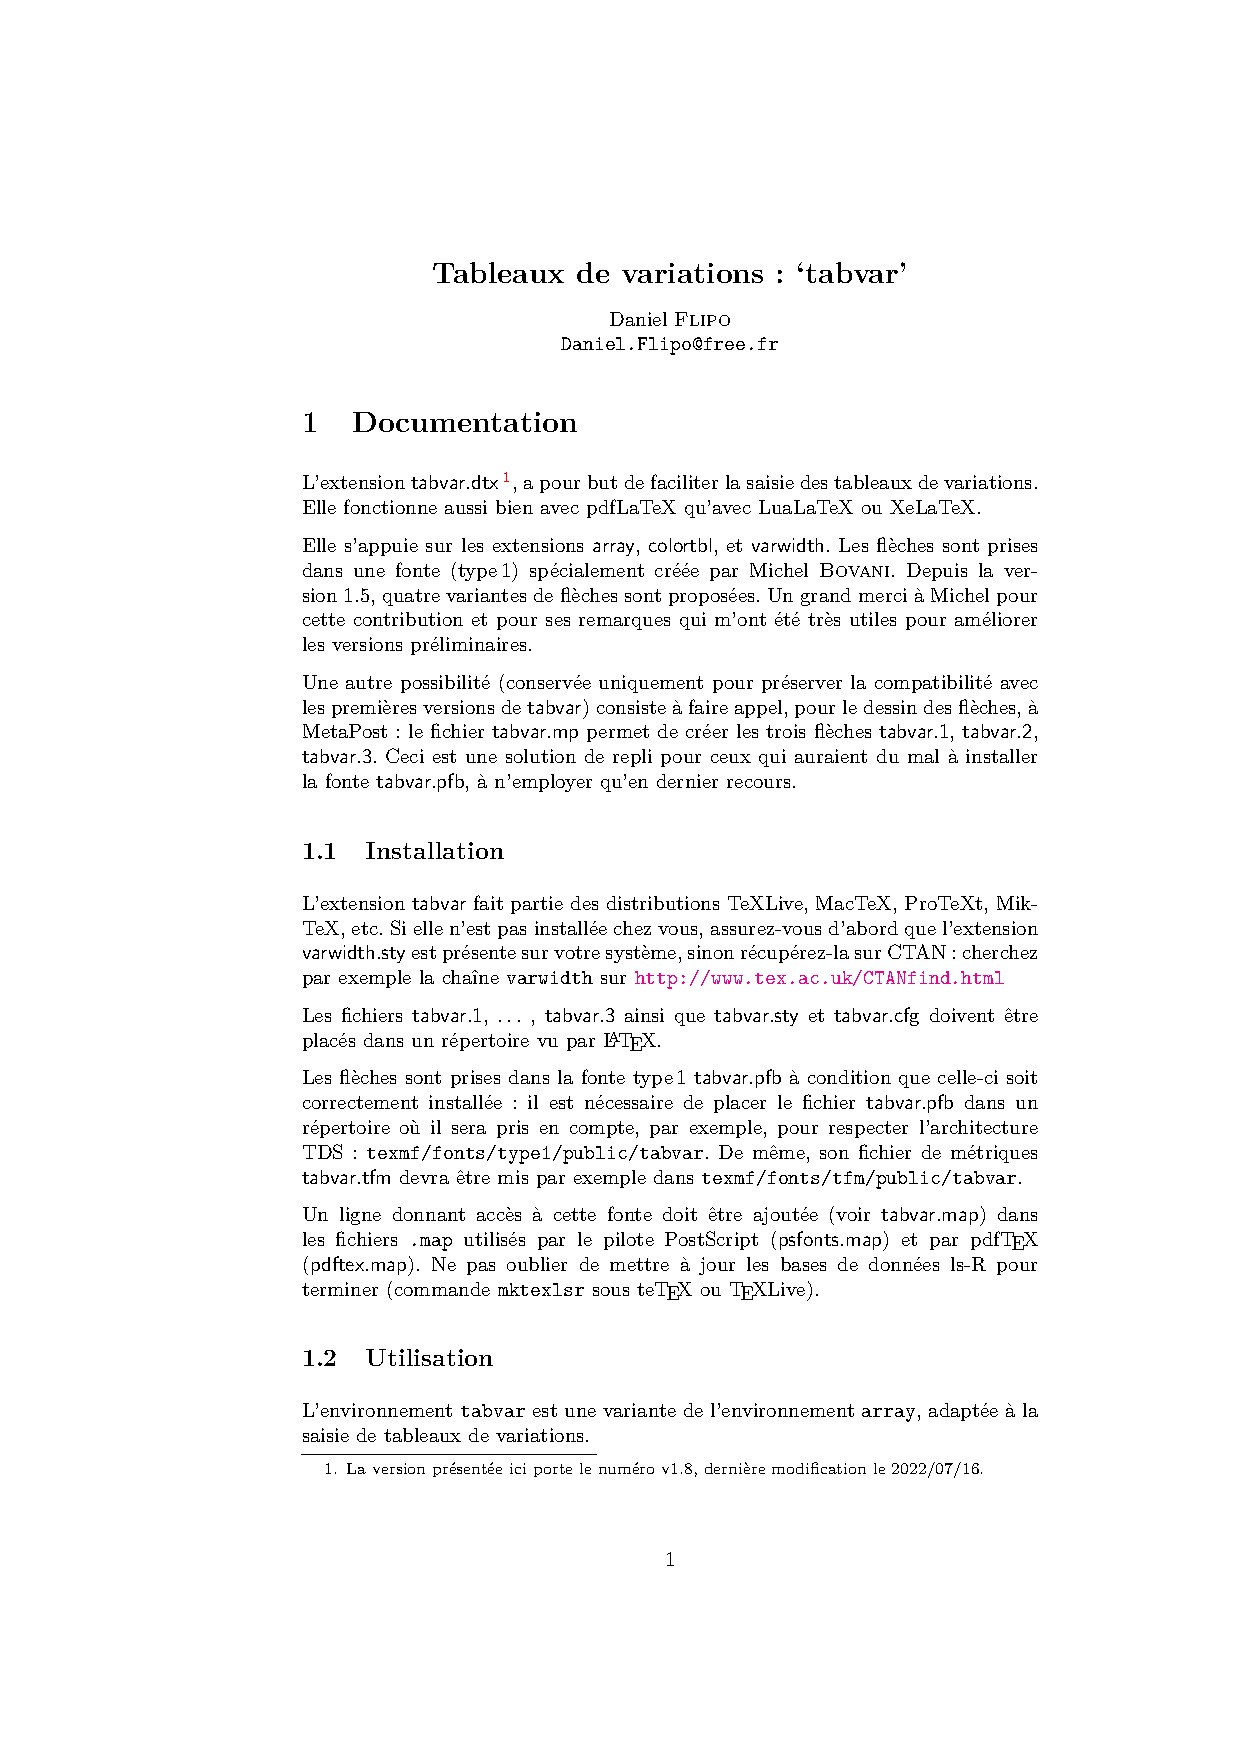
\includegraphics[scale=\TVarrowscale]{tabvar.3}}%
    \newcommand*{\FlecheC}{%
        \TV@arrowcol@stretch{\raisebox{.5ex}{\usebox{\arup}}}}%
    \newcommand*{\FlecheD}{%
        \TV@arrowcol@stretch{\raisebox{.5ex}{\usebox{\ardown}}}}%
    \newcommand*{\FlecheH}{%
        \TV@arrowcol@stretch{\raisebox{.5ex}{\usebox{\arhor}}}}%
  \else
    \DeclareFontFamily{U}{tv}{}%
    \DeclareFontShape{U}{tv}{m}{n}{<->tabvar}{}%
    \DeclareSymbolFont{tvsymbols}{U}{tv}{m}{n}%
    \DeclareMathSymbol{\eastarrowi}{\mathrel}{tvsymbols}{"21}%
    \DeclareMathSymbol{\enearrowi}{\mathrel}{tvsymbols}{"25}%
    \DeclareMathSymbol{\esearrowi}{\mathrel}{tvsymbols}{"26}%
    \DeclareMathSymbol{\eastarrowii}{\mathrel}{tvsymbols}{"31}%
    \DeclareMathSymbol{\enearrowii}{\mathrel}{tvsymbols}{"35}%
    \DeclareMathSymbol{\esearrowii}{\mathrel}{tvsymbols}{"36}%
    \DeclareMathSymbol{\eastarrowiii}{\mathrel}{tvsymbols}{"3B}%
    \DeclareMathSymbol{\enearrowiii}{\mathrel}{tvsymbols}{"3F}%
    \DeclareMathSymbol{\esearrowiii}{\mathrel}{tvsymbols}{"40}%
    \DeclareMathSymbol{\eastarrowiv}{\mathrel}{tvsymbols}{"46}%
    \DeclareMathSymbol{\enearrowiv}{\mathrel}{tvsymbols}{"4A}%
    \DeclareMathSymbol{\esearrowiv}{\mathrel}{tvsymbols}{"4B}%
    \newcommand*{\FlecheC}{%
            \TV@arrowcol@stretch{\ensuremath{\enearrow}}}%
    \newcommand*{\FlecheD}{%
            \TV@arrowcol@stretch{\ensuremath{\esearrow}}}%
    \newcommand*{\FlecheH}{%
            \TV@arrowcol@stretch{\ensuremath{\eastarrow}}}%
  \fi}
%    \end{macrocode}
%  \end{macro}
%  \end{macro}
%  \end{macro}
%
%  \subsection{Positionnement vertical de éléments}
%
%    La variable |\TVextraheight|, dont la valeur par défaut vaut
%    |.7\baselineskip| permet d’écarter légèrement les valeurs
%    maximales de la fonction, du filet horizontal supérieur.
%
%    \begin{macrocode}
\newdimen\TVextraheight
\setlength{\TVextraheight}{.7\baselineskip}
%    \end{macrocode}
%
%  \begin{macro}{\niveau}
%    La commande |\niveau|, utilisée uniquement dans les lignes
%    relatives aux valeurs des fonctions, permet d’initialiser les
%    valeurs des compteurs |\@niveaux| (nombre total de niveaux
%    utilisés dans la ligne) et |\@pos| (indicateur du niveau
%    courant). Elle active également le drapeau |\if@socle|
%    utilisé par la commande |\@socle|. Celle-ci place un filet
%    invisible de hauteur |\TVextraheight| et ajoute |\@pos - 1|
%    sauts de lignes (les colonnes sont alignées par le bas), ce
%    qui assure le positionnement vertical de l’élément (valeur
%    de la fonction ou flèche).
%    Le drapeau |\if@socle| devra être mis localement à `faux’
%    dans certaines colonnes (cf. |\dbarre| et |discont|).
%    \begin{macrocode}
\newcount\@niveaux
\newcount\@pos
\newif\if@socle
\newcommand{\niveau}[2]{\global\@pos=#1 \global\@niveaux=#2
                        \global\@socletrue}
\newcommand{\@socle}{%
  \ifnum\@pos=1 \@soclefalse \fi
  \if@socle
    \rule{\z@}{\TVextraheight}%
    \@tempcnta=\@pos
    \advance\@tempcnta by -1
    \whiledo{\@tempcnta>0}{\TVnl \null \advance\@tempcnta by -1}%
  \fi}
%    \end{macrocode}
%  \end{macro}
%
%  \subsection{Nouveaux types de colonnes}
%
%    Ces définitions nécessitent les extensions |array| et
%    |varwidth|. L’environnement |varwidth|, comme |minipage|,
%    redéfinit la commande |\\|.  On la renomme à l’intérieur
%    des environnements |varwidth|, de façon à éviter la
%    confusion entre passage à la ligne à l’intérieur d’une
%    colonne et passage à la ligne suivante du tableau :
%    |\TVnl| (commande interne) provoque un changement de ligne à
%    l’intérieur d’une colonne, l’utilisateur peut continuer à
%    utiliser |\\| pour terminer une ligne du tableau.
%    La commande |\TVtabularnewline|, définie dans l’environnement
%    \env{tabvar}, provoque un changement de ligne dans le tableau
%    (|\tabularnewline|) et affecte la valeur `vrai’ au drapeau
%    |\ifreset@niveaux|, ce qui commande la réinitialisation des
%    compteurs |\@pos| et |\@niveaux| à la valeur~1.
%    Cette réinitialisation aura lieu \emph{après} que la
%    commande |\@socle| ait placé les valeurs de la fonction et
%    les flèches à la bonne hauteur.
%
%    \begin{macrocode}
\newif\ifreset@niveaux
\newcommand{\reset@niveaux}{%
  \ifreset@niveaux
    \global\@niveaux=1 \global\@pos=1 \global\@soclefalse
  \fi}
%    \end{macrocode}
%
% \changes{tabvar-1.0}{2006/03/14}{Ajout d’un paramètre
%    \cs{TVmaxcolwidth} pour choisir la largeur maximale des colonnes
%    de type C, L, R, au lieu d’une valeur fixe.}
%
% \changes{tabvar-1.2b}{2009/10/03}{Augmenter la valeur de
%    \cs{TVmaxcolwidth} à \cs{linewidth}).}
%
%    On définit des variantes \ctype{C}, \ctype{L} et \ctype{R},
%    des colonnes \ctype{c}, \ctype{l} et \ctype{r} : ce sont des
%    \emph{minipage} alignées par le bas, dont la largeur est celle
%    de la ligne la plus longue, avec un maximum de |\TVmaxcolwidth|
%    fixé à |\linewidth| par défaut, (voir la documentation de
%    l’extension \file{varwidth.sty}).
%
%    \begin{macrocode}
\newdimen\TVmaxcolwidth
\setlength{\TVmaxcolwidth}{\linewidth}
\newcolumntype{C}{%
   >{\begin{varwidth}[b]{\TVmaxcolwidth}\let\TVnl=\\
     \let\\=\TVtabularnewline $}%
   c%
   <{\@socle \reset@niveaux
     $\@finalstrut\@arstrutbox\end{varwidth}}}
\newcolumntype{L}{%
   >{\begin{varwidth}[b]{\TVmaxcolwidth}\let\TVnl=\\
     \let\\=\TVtabularnewline $}%
   l%
   <{\@socle \reset@niveaux
     $\@finalstrut\@arstrutbox\end{varwidth}}}
\newcolumntype{R}{%
   >{\begin{varwidth}[b]{\TVmaxcolwidth}\let\TVnl=\\
     \let\\=\TVtabularnewline $}%
   r%
   <{\@socle \reset@niveaux
     $\@finalstrut\@arstrutbox\end{varwidth}}}
%    \end{macrocode}
%
%\changes{tabvar-1.6}{2011/07/07}{Ajout du type `U’ synonyme de `N’
%    utilisé par numprint.sty. N.B.: c’est la dernière
%    définition qui est prise en compte par \cs{newcolumntype},
%    donc celle de numprint si tabvar est chargé après tabvar
%    et inversement (cf. array.dtx).}
%
%    On définit également un type \ctype{U} pour les domaines où
%    la fonction n’est pas définie : la colonne est coloriée en
%    faisant appel à l’extension \file{colortbl}. La couleur
%    peut être choisie par l’utilisateur, par exemple :\\
%    |\definecolor{TVcolor}{rgb}{0.66, 0.8, 0}| \\
%    donne un vert, voir \file{color.sty} pour la façon de
%    définir des couleurs. L’ancien nom \ctype{N}, conservé pour
%    la compatibilité ascendante, tant qu’il n’y a pas conflit, mais
%    ne devrait plus être utilisé.
%
%    \begin{macrocode}
\definecolor{TVcolor}{gray}{0.7}
\newdimen\TVarraycolsep
\newdimen\TVcolorLeftSep
\newdimen\TVcolorRightSep
\setlength{\TVcolorLeftSep}{\TVarraycolsep}
\setlength{\TVcolorRightSep}{\TVarraycolsep}
\newcolumntype{U}{%
   >{\columncolor{TVcolor}[\TVcolorLeftSep][\TVcolorRightSep]}
   c}
\AtBeginDocument{%
  \@ifundefined{NC@find@N}%
     {\newcolumntype{N}{U}}%
     {\PackageWarning{tabvar}{Le type de colonne N est défini par
                              ailleurs. \MessageBreak Remplacer N par
                              U dans \protect\begin{tabvar}{...N...}
                              \MessageBreak}}%
}
%    \end{macrocode}
%
%  \subsection{Commandes de saisie}
%
%    Les valeurs à afficher dans chaque ligne peuvent être
%    saisies directement (|1.4|, |+|, |-|, etc.) comme dans un
%    tableau normal. Les lignes correspondant aux valeurs des
%    fonctions comportent plusieurs étages, nous disposons
%    deux compteurs, |\@niveaux| qui contient le nombre total
%    de niveaux (ou étages) utilisés dans la ligne, |\@pos|
%    qui indique le niveau courant.
%
%  \begin{macro}{\croit}
%  \begin{macro}{\decroit}
%  \begin{macro}{\constante}
%    Les commandes |\croit|,|\decroit|  et |\constante| tracent les
%    flèches à la hauteur adéquate et mettent à jour le
%    compteur |\@pos|. Un message d’erreur est affiché lorsque
%    l’une de ces commandes fait sortir de la plage de niveaux
%    déclarés par la commande |\niveau|.
%
%    \begin{macrocode}
\newcommand{\decroit}{\FlecheD
                      \global\advance\@pos by -1
                      \ifnum\@pos<1
                      \PackageError{tabvar.sty}%
                        {Les arguments la commande
                         \protect\niveau\space sont incorrects}%
                      \fi}
\newcommand{\croit}  {\raisebox{-\baselineskip}{\FlecheC}%
                      \global\advance\@pos by 1
                      \ifnum\@pos>\@niveaux
                      \PackageError{tabvar.sty}%
                        {Les arguments la commande
                         \protect\niveau\space sont incorrects}%
                      \fi}
\newcommand{\constante}{\FlecheH}
%    \end{macrocode}
%  \end{macro}
%  \end{macro}
%  \end{macro}
%
% \changes{tabvar-1.1}{2007/05/07}{Ajout de la commande \cs{barre}.
%   Ajout de \cs{barre@dth} pour le calcul de la hauteur d’une
%   rangée (utilisée par \cs{barre} et \cs{dbarre}).}
%
%  \begin{macro}{\dbarre}
%    La commande |\dbarre| sert à tracer les doubles barres
%    La commande |\vline| ne peut pas être utilisée à cette fin
%    dans les environnements de type |\parbox|, car sa portée
%    est limitée à un interligne.
%
%    On calcule la hauteur exacte de la rangée, dans les deux cas
%    |\@niveaux=1| et |\@niveaux>1|, |\@tempdimc| contient la hauteur
%    totale (\textit{totalheight}) et |\@tempdimb| la profondeur
%    (\textit{depth}).
%    \begin{macrocode}
\newcommand{\barre@dth}{%
   \ifnum\@niveaux=1
     \@tempdimc=\TVarraystretch\baselineskip
   \else
     \@tempcnta=\@niveaux
     \advance\@tempcnta by -1
     \@tempdimc=\@tempcnta\baselineskip
     \@tempdimb=\TVextraheight
     \ifdim\@tempdimb<.7\baselineskip
       \@tempdimb=.7\baselineskip
     \fi
     \advance\@tempdimc by \@tempdimb
     \advance\@tempdimc by \dp\@arstrutbox
   \fi
   \@tempdimb=\dp\@arstrutbox}
%    \end{macrocode}
%    On fait appel à |\rule| pour le tracé de |\dbarre|.
%    \begin{macrocode}
\newcommand{\dbarre}{%
   \barre@dth
   \rule[-\@tempdimb]{.5\p@}{\@tempdimc}%
   \kern 2\p@
   \rule[-\@tempdimb]{.5\p@}{\@tempdimc}%
   \@soclefalse}
%    \end{macrocode}
%  \end{macro}
%
%\changes{tabvar-1.3}{2010/04/03}{%
%  Valeur de la profondeur \cs{@tempdimb} corrigée dans \cs{barre}.
%  Bug signalé par Frank Stengel.}
%
%  \begin{macro}{\barre}
%    La commande |\barre| prend un argument obligatoire.
%    |\barre{}| trace un filet vertical centré dans une colonne.
%    Lorsque l’argument est non vide, celui-ci est superposé
%    (centré) sur le filet. Le filet est tracé en gris
%    par défaut (couleur paramétrable).
%    \begin{macrocode}
\newsavebox{\tab@box}
\definecolor{TVbarrecolor}{gray}{0.7}
\newcommand{\barre}[1]{%
   \sbox{\tab@box}{\ensuremath{#1}}%
   \barre@dth
   \@tempcnta=\@pos
   \advance\@tempcnta by -1
   \advance\@tempdimb by \@tempcnta\baselineskip
   \raisebox{-\@tempdimb}[0pt][0pt]{%
      \makebox[\wd\tab@box][c]{\color{TVbarrecolor}%
                               \rule{.5\p@}{\@tempdimc}}}%
   \kern-\wd\tab@box\usebox{\tab@box}%
}
%    \end{macrocode}
%  \end{macro}
%
%  \begin{macro}{\discont}
%    La commande |\discont| s’utilise lorsque la fonction présente
%    une discontinuité, elle réclame 3 arguments obligatoires :
%    le premier est la limite à gauche~$f_-$, le deuxième le signe
%    `<’ ou `>’, le troisième est la limite à droite~$f_+$.
%    \LaTeX{} ne peut pas toujours comparer facilement les valeurs
%    de $f_-$ et $f_+$ (penser à $f_-=\sqrt{e}$, $f_+=\pi/2$), le
%    deuxième argument précise si $f_- < f_+$ ou si $f_- > f_+$.
%
%    En plus de ces 3 arguments obligatoires, un argument optionnel
%    (entier positif) permet d’écarter verticalement les valeurs
%    $f_-$ et~$f_+$ ; la valeur de cet entier donne le nombre de
%    niveaux supplémentaires à intercaler (0 par défaut).
%
%    On commence par mesurer la largeur des deux arguments |#2| et
%    |#4| pour pouvoir les centrer ensuite dans une boîte de
%    largeur égale au maximum des deux largeurs.
%    Si cette disposition ne convient pas, on pourra toujours
%    ajouter un |\hfill| à droite où à gauche de la valeur
%    à déplacer.
%
%    \begin{macrocode}
\newcommand{\discont}[4][0]{%
     \settowidth{\@tempdimc}{\ensuremath{#2}}%
     \settowidth{\@tempdimb}{\ensuremath{#4}}%
     \ifdim\@tempdimc<\@tempdimb \@tempdimc=\@tempdimb\fi
     \rule{\z@}{\TVextraheight}%
     \@soclefalse
     \ifthenelse{\equal{#3}{<}}%
%    \end{macrocode}
%    Cas où $f_- < f_+$ : on pose la valeur de~$f_+$ (|#4|), puis
%    on saute autant de lignes supplémentaires qu’indiqué dans
%    l’argument optionnel, ensuite on passe à la ligne et on pose
%    la valeur de~$f_-$ (|#2|), enfin on ajoute en dessous
%    |\@pos - 1| sauts de lignes pour positionner le tout en hauteur.
%    Il reste à ajuster le compteur~|\@pos| pour que la flèche
%    suivante soit placée à la bonne hauteur.
%    \begin{macrocode}
     {\makebox[\@tempdimc]{\ensuremath{#4}}%
      \@tempcnta=#1
      \whiledo{\@tempcnta>0}{\TVnl \null \advance\@tempcnta by -1}%
      \TVnl
      \makebox[\@tempdimc]{\ensuremath{#2}}%
      \@tempcnta=\@pos
      \advance\@tempcnta by -1
      \whiledo{\@tempcnta>0}{\TVnl \null \advance\@tempcnta by -1}%
      \global\advance\@pos by 1
      \global\advance\@pos by #1
     }%
     {\ifthenelse{\equal{#3}{>}}%
%    \end{macrocode}
%    Cas où $f_- > f_+$ : \textit{idem} en permutant $f_-$ et~$f_+$.
%    \begin{macrocode}
     {\makebox[\@tempdimc]{\ensuremath{#2}}%
      \@tempcnta=#1
      \whiledo{\@tempcnta>0}{\TVnl \null \advance\@tempcnta by -1}%
      \TVnl
      \makebox[\@tempdimc]{\ensuremath{#4}}%
      \@tempcnta=\@pos
      \advance\@tempcnta by -2
      \advance\@tempcnta by -#1
      \whiledo{\@tempcnta>0}{\TVnl \null \advance\@tempcnta by -1}%
      \global\advance\@pos by -1
      \global\advance\@pos by -#1
     }%
%    \end{macrocode}
%    Cas où le deuxième argument n’est ni |<| ni |>| : erreur
%    \begin{macrocode}
     {\PackageError{tabvar.sty}%
        {Le second argument de \protect\discont\space doit être
         \MessageBreak soit '<' soit '>'}}%
     }%
}
%    \end{macrocode}
%  \end{macro}
%
%\changes{tabvar-1.6}{2011/07/07}{Ajout de la commande \cs{TVcenter}.}
%
%  \begin{macro}{\TVcenter}
%    La commande |\TVcenter{}| prend un argument, le nom de la
%    fonction à centrer verticalement dans sa colonne.
%    \begin{macrocode}
\newcommand*{\TVcenter}[1]{%
  \@tempcnta=\@niveaux \advance\@tempcnta by -1 \divide\@tempcnta by 2
  \@tempdimb=\@tempcnta\baselineskip
  \ifodd\@niveaux\else\advance\@tempdimb by .5\baselineskip\fi
  \@pos=1\raisebox{\@tempdimb}{\ensuremath{#1}}%
}
%    \end{macrocode}
%  \end{macro}
%
%\changes{tabvar-1.7}{2012/12/23}{Ajout de la commande \cs{TVstretch}.}
%
%  \begin{macro}{\TVstretch}
%    La commande |\TVstretch{}| prend un argument obligatoire, le nom
%    de la valeur à écarter des lignes horizontales et un
%    argument optionnel de type \emph{dimension}.
%    Elle place son argument dans une boîte et en mesure la hauteur
%    et la profondeur. En l’absence d’argument optionnel, elle ajoute
%    respectivement |\TVextraheight| à la hauteur |\TV@tempa| et
%    |\TVextradepth| à la profondeur |\TV@tempb|.
%
%    Si l’argument optionnel est une dimension positive, sa valeur
%    sera ajoutée uniquement à la hauteur et si c’est une
%    dimension négative sa valeur absolue sera ajoutée uniquement
%    à la profondeur. La valeur par défaut de l’argument optionnel
%    est |0pt|.
%
%    \begin{macrocode}
\newsavebox\TVbox
\newdimen\TVextraheight
\newdimen\TVextradepth
\setlength{\TVextraheight}{2pt}
\setlength{\TVextradepth}{2pt}
\newdimen\TV@tempa
\newdimen\TV@tempb
\newcommand{\TVstretch}[2][0pt]{%
  \edef\tmp{#1}%
  \sbox{\TVbox}{\ensuremath{#2}}%
  \settoheight{\TV@tempa}{\usebox{\TVbox}}%
  \settodepth {\TV@tempb}{\usebox{\TVbox}}%
  \ifdim\tmp=0pt
    \addtolength{\TV@tempa}{\TVextraheight}%
    \addtolength{\TV@tempb}{\TVextradepth}%
  \else
    \ifdim\tmp>0pt
      \addtolength{\TV@tempa}{\tmp}%
    \else
      \addtolength{\TV@tempb}{-\tmp}%
    \fi
  \fi
%    \end{macrocode}
%    Il reste à afficher la boîte initiale et à lui adjoindre
%    une |\rule| invisible (de largeur nulle) de profondeur
%    |\TV@tempb| et de hauteur totale |\TV@tempa + \TV@tempb|.
%    \begin{macrocode}
  \usebox{\TVbox}%
  \addtolength{\TV@tempa}{\TV@tempb}%
  \rule[-\TV@tempb]{0pt}{\TV@tempa}%
}
%    \end{macrocode}
%  \end{macro}
%
%  \subsection{Environnement `tabvar’}
%
%    L’environnement \env{tabvar} est un \env{array} où sont
%    redéfinis |\TVarraystretch|, |\TVarraycolsep| et
%    |\tabularnewline|.
%
%  \begin{environment}{tabvar}
%    \begin{macrocode}
\newcommand{\TVarraystretch}{1.5}
\setlength{\TVarraycolsep}{1pt}
\newenvironment{tabvar}[1]
  {\renewcommand{\arraystretch}{\TVarraystretch}%
   \setlength{\arraycolsep}{\TVarraycolsep}%
   \global\@niveaux=1 \global\@pos=1 \global\@soclefalse
   \def\TVtabularnewline{\reset@niveauxtrue\tabularnewline}%
   \begin{array}{#1}}
  {\end{array}}
%    \end{macrocode}
%  \end{environment}
%
%    Chargement du fichier de préférences, si il en existe un.
%    \begin{macrocode}
\InputIfFileExists{tabvar.cfg}
   {\typeout{loading tabvar.cfg}}
   {\typeout{tabvar.cfg not found, using default values}}
%    \end{macrocode}
% \iffalse
%</sty>
% \fi
%
%  \section{Fichier de configuration}
%
% \iffalse
%<*cfg>
% \fi
%    \begin{macrocode}
%% Fichier de configuration de l’extension `tabvar.sty’.
%%
%% Décommenter la ligne suivante pour que les variantes MetaPost
%% des flèches soient utilisées à la place de la fonte tabvar.pfb
%% (déconseillé en général et *jamais* sous LuaLaTeX ou XeLaTeX).
%%
%%\FlechesMPtrue
%%
%% Choix d’une des 4 variantes pour les flèches PostScript
%%
%%\FlechesPS1   % (défaut)
%%\FlechesPS2   % assorties à la police Fourier
%%\FlechesPS3
%%\FlechesPS4
%%
%% Ce paramètre permet d’augmenter la largeur des colonnes contenant
%% des flèches (essayer 1.3, 1.5, etc.), sa valeur par défaut est 1 :
%%
%%\renewcommand*{\TVarrowscolstretch}{1}
%%
%% Ce paramètre permet d’ajuster la hauteur des lignes
%% de `tabvar’ correspondant aux variations d’une fonction ;
%% sa valeur par défaut est :
%%
%%\setlength{\TVextraheight}{0.7\baselineskip}
%%
%% Valeur de \arraycolsep utilisée dans `tabvar’.
%%
%%\setlength{\TVarraycolsep}{1pt}
%%
%% Valeur de \arraystretch utilisée dans `tabvar’.
%%
%%\renewcommand{\TVarraystretch}{1.5}
%%
%% Largeur maximale des colonnes de type C, L ou R.
%%
%%\setlength{\TVmaxcolwidth}{\linewidth}
%%
%% Valeur des espaces verticaux ajoutés par la commande
%% |\TVstretch{}|.
%%
%%\setlength{\TVextraheight}{2pt}
%%\setlength{\TVextradepth}{2pt}
%%
%% Exemples de définitions de couleurs pour les colonnes `U’
%% où la fonction est non définie.
%%
%%\definecolor{TVcolor}{gray}{0.5}
%%\definecolor{TVcolor}{rgb}{0.33, 0.12, 0}
%%\definecolor{TVcolor}{cmyk}{0.91,0,0.88,0.12}
%%
%% Les valeurs suivantes assurent que les colonnes `U’ sont
%% coloriées sur toute leur largeur.
%%
%%\setlength{\TVcolorLeftSep}{\TVarraycolsep}
%%\setlength{\TVcolorRightSep}{\TVarraycolsep}
%%
%% On peut ajuster comme ci-dessus la couleur des filets
%% traçés par la commande \barre{}.
%%
%%\definecolor{TVbarrecolor}{gray}{0.7}
%    \end{macrocode}
% \iffalse
%</cfg>
% \fi
%
% \Finale
%
% \PrintChanges
\endinput

%%% Local Variables:
%%% fill-column: 70
%%% coding: utf-8
%%% End:
